

\chapter{Preliminaries}\label{chap1}

\section{}

IN\pageoriginale THIS CHAPTER, which we offer as an introduction, one
will not find many proofs. The aim is to state clearly some concepts
so that we can speak rigorously of the different ideals defining a
projective embedded variety. We give also the duality theorems and
some of their consequences (finiteness, vanishing and Riemann-Roch
theorem for curves), notions which play the role of `Completeness of a
linear system' or `Specialness of a  divisor'. The reader will find
complete proofs of two intersecting facts:
\begin{itemize}
\item [(i)] There exists a curve in $\mathbb{P}^3$ with no imbedded
smooth deformation. 
\item [(ii)] Every curve in $\mathbb{P}^3$ which is locally a complete
  intersection can be defined by four equations.
\end{itemize}
For simplicity we throughout assume that the base field is
algebraically closed. 

A {\it graded ring} $A$ is a ring of the form:
$$
A=A_0\oplus A_1\oplus A_2\oplus \ldots,
$$
such that $A_0$ is a ring, $A_i$'s are all $A_0$-modules and $A_i.A_j
\subset A_{i+j}$. Any $f\in A_i$ for some $i$ is said to be a {\it
homogeneous element} of $A$. An ideal I of $A$ is said to be a graded
ideal, if $\Sigma f_i\in I$, with $f_i\in A_i$ (\ie $f_i$ homogeneous)
then $f_i\in I$. 

Assume $A_0$ is a field and also $A$ is generated by $A_1$ over
$A_0$. $A_1$ a finite dimensional vector space over $A_0$. We define
$X=\Proj A$ as follows: Set theoretically $X=\{\text{All graded prime
ideals of}\quad A\neq A_1\oplus A_2\oplus\ldots\}$. 

We will give $X$ a scheme structure, by covering $X$ by affine open
sets: Let\pageoriginale $f\in A_1$. Then,
\begin{equation}
A_f=(A_f)_0[T, T^{-1}],\tag{*}
\end{equation}
where $(A_f)_0=\left\{\dfrac{g}{f^n} \; g\in A_n \right\}$. (degree $0$ elts. in $A_f$.)

$(A_f)_0$ is clearly a ring with identity.

\noindent $(*)$ is got by mapping $T$ to $f$ and $T^{-1}$ to $f^{-1}$
in $A_f$. Denote by $X_f$ the set $\{p\in X/f\notin p\}$,
clearly there is a canonical bijection
$$
X_f\leftrightarrow\Spec(A_f)_0.
$$

Transferring the scheme structure to $X_f$ and verifying that this
structure is compatible as we vary $f\in A_1$, we get a scheme
structure on $X$.
\begin{example*}
\begin{itemize}
\item [1.] Let $A=K[X_0,X_1\ldots X_n]$ be polynomial ring in $n+1$ variables
graded in the natural way: $A_0=k.A_1=$ vector space of dimension
$n+1$ with $X_0,\ldots,X_n$ as generators \ie $A_1=$ set of all
homogeneous linear polynomials in $X_i$'s. $A_n=$ set of all
homogeneous polynomials in 
$$
X_i\text{'s of}\deg n.
$$

Then $\Proj A=\mathbb{P}^n$, the projective space of dimension $n$.
\item [2.] Let $I$ be any ideal of $A$ generated by homogeneous
polynomials $\{f_1,\ldots,f_n\}$. Then $A'=A/I$ is a graded ring
$X=\Proj A'$ and $\Proj A=\mathbb{P}^n:X$ is the closed subvariety
of $\mathbb{P}^n$ defined by equations $(f_1,\ldots,f_n)$.

$M=\underset{n\in\mathbb{Z}}{\oplus}M_n$ is said to be a {\it graded
$A$-module} over the graded ring $A=\underset{i\geq 0}{\oplus}A_i$
if $M$ is an $A$-module and $A_i.M_n\subset M_{n+i}$. 

If $M$ ia a graded $A$-modale we can associate a sheaf $\tilde{M}$ to
$M$ over $X=\Proj A$ as follows: Over $X_f$ we define the sheaf to be
$(M_f)_0$ where $(M_f)_0$ is\pageoriginale the set of degree zero
elements of $M_f$. It is a module over $(A_f)_0$. [Recall that
$X_f=\spec(A_f)_0$]. One can check that this defines a sheaf over
$X$. 
\end{itemize}
\end{example*}

\begin{REM*}
$\tilde{A}=O_X$.

If $M$ is a graded $A$-module, we define $M(n)$ to be the graded
$A$-module given by, $M(n)_k=M_{n+k}$. We denote $\widetilde{M(n)}$ by
$\tilde{M}(n)$. In particular.
$$
\widetilde{A(n)}=\tilde{A}(n)=O_X(n).
$$

If $F$ is any sheaf on $X$, we denote by $F(n)$ the sheaf
$F\otimes_{O_X}O_X(n)$. If $X=\Proj A$, then $Y=\spec A$ is defined to
be a {\it cone} over $X$.


et $P$ denote the point in $Y$ corresponding to the special maximal
ideal $A_1\oplus A_2\oplus\ldots P$ is defined as the {\it vertex} of
the cone $Y$ over $X$.
\begin{figure}[H]
\centering
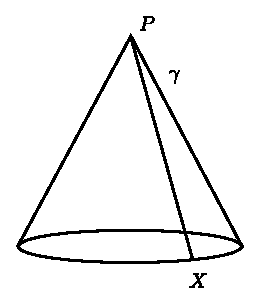
\includegraphics{figure/addfig1.eps}
\end{figure}


Let $I$ be any graded ideal of $A$. Then $A/I$ is a graded
ring. Denote by $Z$, the scheme $\Proj A/I$. It can be easily checked
that the canonical map $A\longrightarrow A/I$ induces a closed
immersion $Z\rightarrow X=\Proj A$. Conversely given a closed
subscheme $Z$ of $X$, we can find a graded ideal $I\subset A$, such
that the canonical map $\Proj A/I\longrightarrow X$ is an isomorphism
of $\Proj A/I$ with $Z$. Then we say that $I$ {\it ideally defines}
$Z$ in $X$. But this $I$ is not completely determined by $Z$. One can
check that if $I$ is any ideal defining $Z$, then so does $Im^n$
where $m$ corresponds to the special maximal ideal of $A$. (\ie it
corresponds to the vertex of the given cone)

Since we are assuming that $A_0=k$ is a field and $A$ is generated by
$A_1$ over $k$, where $A_1$ is finite dimensional over $k$, we have a
graded ring homomorphism,\pageoriginale
$$
R=k[X_0, X_1,\ldots X_n]\longrightarrow A,
$$
which is surjective. [Polynomial rings have the canonical
  grading]. The kernel is a graded ideal $J$ in $R$. So we have a
closed immersion $X=\Proj A\hookrightarrow\Proj R=\mathbb{P}_k^n$.

Thus all the schemes we have considered are closed subschemes in some
$\mathbb{P}_k^n$ (In particular they are all projective).
\end{REM*}

\begin{REM*}
We have already seen that $J$ need not be unique. But if $X$ is
reduced and if we insist that $R/J$ is also reduced then $J$ is
unique. [Take $J=$ root ideal of any ideal defining $X$].

If $X=\Proj R/J,\ie J$ is some ideal of $R$ defining $X$ then using
(*) one can verify that $\spec R/J-[P]$ is uniquely determined. In
other words any ideal $J$ which defines $X$ ideally determines the
corresponding cone everywhere except the vertex.
\end{REM*}

\begin{examples*}
\begin{itemize}
\item [1.] Let $R=k[X_0, X_1]$. So $\Proj R=\mathbb{P}_k^1$.

Let $J_1=(X_0)$ and $J_2=(X_0^2,X_0X_1)$. Then $\Proj R/J_1\cong\Proj
R/J_2.\break J_1\underset{\neq}{\supset}J_2$. Note that $(R/J_1)_P$ is
Cohen-Macaulay $(\because\depth(R/J_1)_P=1)$ and $\depth(R/J_2)_P=0$,
where $P$ is the vertex.
\item [2.] Take the imbedding of $\mathbb{P}^1$ in $\mathbb{P}^3$
given by: $(x_0,x_1)\longrightarrow
(x_0^3,x_0^2x_1,\break x_0x_1^2,x_1^3)$. Then an ideal defining the image in
$\mathbb{P}^3$ is
$J=(X_0X_3-X_1X_2,X_0X_2-X_1^2,X_1X_3-X_2^2)$. We see that the variety
is not a complete intersection and the vertex of the cone is also not
a complete intersection. We\pageoriginale will show now how properties
of the vertex affect the variety itself.
\end{itemize}
\end{examples*}

\begin{propn}\label{chap1:prop1.1}
Let $A=k\oplus A_1\oplus A_2\oplus\ldots$ be a graded ring where $A_1$
is a finitely generated vector space over $k$ generating $A$ as a
graded $k$-algebra. Let $P$ be the vertex. Then
\begin{itemize}
\item [i)] $A_P$ is $R_i\Longrightarrow\Proj A$ is $R_i$
\item [ii)] $A_P$ is $S_i\Longrightarrow\Proj A$ is $S_i$
\item [iii)] $A_P$ is a complete intersection $\Longrightarrow\Proj A$
  is locally completely intersection
\item [iv)] $A_P$ is a $U.F.D\Longrightarrow A$ is factorial
\end{itemize}
\end{propn}

\begin{proof}
Assume that $A_P$ has \#. Let \# denote any of the properties (i),
(ii), (iii). Since $\Proj A$ is covered by open sets of the type
$\Spec A_{(f)_\circ},f\in A_1$, it suffices to prove that \# holds for
each one of them.

So let $p\in\Spec A_{(f)_{\circ}}$. We want to show that
$(A_{(f)_{\circ}}p$ has \# But ${(A_{(f)_{\circ}}}_p$ has
$\#\Longleftrightarrow A_{(f)_\circ}[T,T^{-1}]_{p[T,T^{-1}]}$ has
  \#.

As we have already seen $A_{(f)_\circ}[T,T^{-1}]\simeq A_f$ and then
$p[T,T^{-1}]$ will correspond to a prime ideal $qA_f$,
($q\hookrightarrow A$ a homogeneous prime ideal.) So it suffices to
show that \# holds for $A_{f(qA_f)}$. Now $q$ is contained in $P$,
since $q$ is homogeneous and $A_{f(qA_f)}\simeq A_{P_{(qAP)}}$. The
  result then follows from the fact that $A_P$ has \# and hence any
  localization of $A_P$ also has \#. As iv) is easy we leave it to the reader.
\end{proof}

\section{Cohomology of Coherent Sheaves:}\label{chap1:sec2}
Let\pageoriginale $R=k[X_0,\ldots,X_n]$.
Then to any coherent sheaf $\mathcal{F}$ on
$\mathbb{P}^n$, one can associate a graded $R$-module $F$ of finite
type. This correspondence is not unique. But given a graded $R$-module
$F$, we can associate to it a unique sheaf on $\mathbb{P}^n$. For the
definition of cohomology and results on cohomology we refer the reader
to $FAC$ by J.P. Serre and local cohomology by A. Grothendieck. We
denote by $O_{\mathbb{P}^n}(1)$ the line bundle got by hyperplane in
$\mathbb{P}^n$. 
\begin{REM*}
$O_{\mathbb{P}^n}(-1)=\Hom(O_{\mathbb{P}^n}(1),O_{\mathbb{P}^n})=
(O_{\mathbb{P}^n}(1))^v$.  
\end{REM*}

\begin{propn}\label{chap1:prop2.1}
There is an exact sequence for any graded $R$-module $M$
\begin{gather*}
0\longrightarrow H_P^0(M)\longrightarrow M\longrightarrow
\underset{m\in\mathbb{Z}}{\oplus}H^0(\mathbb{P}^n,\tilde{M}(m))
\longrightarrow H_P^1(M)\longrightarrow 0,\\
\text{and}\qquad H_P^{i+1}(M)=\underset{m\in\mathbb{Z}}{\oplus}H^i
(\mathbb{P}^n,\tilde{M}(m)) \; i\geq 1.
\end{gather*}
\end{propn}

\begin{proof}
This statement is almost the same as Prop. 2.2 in
LC. Putting $X=\Spec R$ and $P=Y$ in that result we get
$$
0\longrightarrow H_P^0(M)\longrightarrow M\longrightarrow H^0(\Spec
R-\{P\},\tilde{M})\longrightarrow H_P^1(M)\longrightarrow 0,
$$
where $\tilde{M}$ is the sheaf defined by $M$ on $\Spec R-P$ and 
$$
H_P^{i+1}(M)\cong H^i(\Spec R-P,\tilde{M}),i>0.
$$

So we only have to check that $H^i(\Spec R-P,\tilde{M})\cong
\underset{m}{\oplus}H^i(\mathbb{P}^n,M(m))$, for every $i$,
canonically. We have a map $\Spec R-P\xrightarrow{p}\mathbb{P}^n$
which is a surjection and an affine map. So
$$
H^i(\mathbb{P}^n,p_*\tilde{M})\longrightarrow H^i(\Spec R-P,
\tilde{M}).
$$

So we want to show that,
$$
H^i(\mathbb{P}^n,p_*\tilde{M})=\underset{m}{\oplus}H^i(\mathbb{P}^n,M(m)),
\quad \forall_i.
$$\pageoriginale

But one checks that 
$$
p_*M=\underset{m}{\oplus}\tilde{M}(m)
$$
canonically and the result follows.
\end{proof}

\begin{example*}
$\tilde{M}=O_C$, where $C$ is a reduced curve in $\mathbb{P}^n.
M=R/J.J$ is an ideal defining $C$.
$$
R/J=\oplus H^0(\mathbb{P}^n,R/J(m))=\oplus H^0(\mathbb{P}^n,O_C(m))
$$
where $O_C(m)=O_C(1)^{\otimes_m}$ and $O_C(1)=O_{\mathbb{P}^n}(1)/C$
$$
\oplus H^0(\mathbb{P}^n,O_C(m))=\oplus H^0(C,O_C(m)).
$$
\end{example*}

\begin{claim*}
The map $R/J\longrightarrow\oplus H^0(C,O_C(m))$ is injective if $J$
is the biggest ideal defining $C$.

From the above exact sequence, we get 
\begin{quote}
if $R/J\longrightarrow\oplus H^0(C, O_C(m))$ is injective\\
then $H_P^0(R/J)=0\ie\depth_PR/J\geq 1$. (By Theorem 3.8 of LC.)\\
then $P$ is not an imbedded component\\
hence $J$ is the biggest ideal defining $C$.
\end{quote}
\end{claim*}

\begin{claim*}
If $C$ is a smooth curve,
$$
R/J\longrightarrow\underset{m}{\oplus}H^0(C,O_C(m))
$$
is surjective if and only if $C$ is arithmetically normal.

\noindent By the above exact sequence

\begin{itemize}
\item $R/J\longrightarrow\oplus H^0(C,O_C(m))$\pageoriginale is
injective and surjective
\item $H_P^0(R/J)=H_P^1(R/J)=0\depth_PR/J\geq 2$ by Th.~3.8 of LC
\end{itemize}
since $\Spec R/J-[P]$ is normal we have to check normality only at
$P$. Since $P$ is of codim 2 in $\Spec R/J,(R/J)_P$ is normal by
Serre's criterion.

$\ie C$ is arithmetically normal
\end{claim*}

\section{Vanishing Theorem and Duality}\label{chap1:sec3}

{\bf Vanishing Theorem (Serre).} Let $\mathcal{F}$ be a coherent sheaf
on $\mathbb{P}^n$ Then for all $i>0,
H^i(\mathbb{P}^n,\mathcal{F}(m))=0$ and
$H^0(\mathbb{P}^n,\mathcal{F}(m))$ generate $\mathcal{F}(m)$ as
$O_{\mathbb{P}^n}$ module for $m\gg 0$. 

\medskip
\noindent {\bf Duality Theorem.} Let $\mathcal{F}$ be a locally free
sheaf on $\mathbb{P}^n$, of finite
type. $\omega_{\mathbb{P}^n} = \overset{n}{\Lambda}
\Omega_{\mathbb{P}^n/k}$, where $\Omega_{\mathbb{P}^n/k}^1$ is the
sheaf of differentials. So
$\omega_{\mathbb{P}^n}=O_{\mathbb{P}^n}(-n-1)$. Then $H^i
(\mathbb{P}^n,\mathcal{F})\times H^{n-i}(\mathbb{P}^n,\mathcal{F}
\otimes\omega)\longrightarrow H^n(\mathbb{P}^n,\omega)\simeq k$ is a
perfect pairing.

\medskip
\noindent {\bf Duality on a Locally Cohen-Macaulay Curve $C$:} Let
$\mathcal{F}$ be a locally sheaf of finite rank on $C\hookrightarrow
\mathbb{P}^n$. Then,

$H^i(C,\mathcal{F})\times H^{1-i}(C,\mathcal{F}^v\otimes\omega_C)
\xrightarrow{\sim}H^1(C,\omega_C)$ is a perfect pairing,
with $\omega_C=\underline{\Ext}_{\mathbb{P}^n}^{n-1}
(O_C,\omega_{\mathbb{P}^n})$. 
\begin{itemize}
\item [1.] If $X$ is smooth, $\omega_X=\overset{\max}{\Lambda}
\Omega_{X/k}^1$. 
\item [2.] Let $X$ and $Y$ be equidimensional locally Cohen-Macaulay
  varieties with $X\hookrightarrow Y$. If $c$ is the codimension of
  $X$ in $Y$, then
$$
\omega_X=\underline{\Ext}^c(O_X,\omega_Y).
$$

\begin{Coro*}
If $X$ and $Y$ are as above with $X$ a divisor on $Y$, then $(L\otimes
\omega_Y)_{|X}=\omega_X$ where $L$ is the line bundle associated to
the divisor $X$.
\end{Coro*}

\item [3.] Let\pageoriginale $X$ and $Y$ be equidimensional locally
  Cohen-Macaulay varieties with a finite surjective morphism
  $X\xrightarrow{f}Y$. Then
$$
f_*\omega_X=\underline{\Hom}_{O_Y}(f_*O_X,\omega_Y).
$$
\item [4.] Let $Y$ be a locally Cohen-Macaulay
  variety. $\mathbb{P}_Y^n=\mathbb{P}^n \underset{k}{\times}Y,
\mathbb{P}_Y^n\longrightarrow Y$ be the projection. Then 
$$
\omega_{\mathbb{P}_Y^n}=\pi^*\omega_Y\otimes O_{\mathbb{P}_Y^n}(-n-1).
$$
\end{itemize}

The above results can be found in either of the following: $FAC$ by
J.P. Serre or Introduction to Grothendieck Duality Theory, A. Altman
and S. Kleiman.
\begin{example}\label{chap1:exm1}
If $C$ is a local complete intersection $\omega_C$ is a line bundle.
\end{example}

\begin{example}\label{chap1:exm2}
If $C$ is smooth $\omega_C=\Omega_{C/k}^1$. 
\end{example}

\section{Divisors, Line Bundles and Riemann-Roch
  Theorem.}\label{chap1:sec4} Let $X$ be a scheme, $O_X$ its
structures sheaf, $K_X$ the sheaf of meromorphic functions on
$X,O_X^*$ the sheaf of units of $O_X,K_X^*$ the sheaf of units of
$K_X$. We call a collection $[f_i,U_i]$ where $U_i$'s are affine open
in $X$ and $f_i\in\Gamma(U_i,K^*)$, {\it Cartier Divisor} on $X$ if
$f_if_j^{-1}\in\Gamma(U_i\cap U_j,O_X^*)$.
\begin{example*}
If we take $f_i=1,\quad\forall_i$, then this line bundle is precisely
$O_X$. 

For a more detailed description of divisors and line bundles the
reader can refer to almost any of the Geometry books; for instance
D. Mumford, ``Lectures on Curves on an Algebraic Surface''.

Let $C\longrightarrow\mathbb{P}^n$ be a locally complete
intersection-curve in $\mathbb{P}^n$. Let $C$ be reduced and
connected. Let $L$ be a line bundle on $C$.
$$
\chi (L)=\dim H^0(C,L)-\dim H^1(C,L).
$$

$p=\dim H^1(C,O_C)=\dim H^0(C,\omega_C)$ is called the {\it arithmetic
  genus}. We define degree of line bundle to be,
$$
d^\circ L=\chi(L)- \chi(O_C).
$$\pageoriginale
\end{example*}

\begin{RRochthm*}\label{chap1:RRthm}
$d^\circ L$ is additive \ie $d^\circ(L\otimes M)=d^\circ L+d^\circ
M$. 

Let $D\hookrightarrow C$ be a closed subschem locally defined by one
equation which is a non-zero divisor. Then $D$ is an effective Cartier
divisor. If $J_D$ is its ideal we have the following exact sequence
$$
0\longrightarrow J_D\longrightarrow O_C\longrightarrow O_D
\longrightarrow 0.
$$
and $J_D$ is a line bundle.
\end{RRochthm*}

\begin{def*}
$J_D=O_C(-D)$.
$$
d^\circ O_C(1)=d^\circ (C),\quad\text{if}\quad C\longrightarrow
\mathbb{P}^3\quad\text{is a curve}.
$$

If $C$ is a $\proj$ Curve of $\deg d$ in $\mathbb{P}^2$, then, 
$$
p=\frac{(d-1)(d-2)}{2}
$$
For a proof of this fact see `Elements of the Theory of Algebraic
Curves' by A. Seidenberg, pp.~118. If $g$ is the geometric genus of
$C$, then $p\geq g$.
\end{def*}

\begin{bezout'sthm*}\label{chap1:bezthm}
If $X,Y\hookrightarrow\mathbb{P}^n \proj$ varieties imbedded in
$\mathbb{P}^n \dim X=r,\dim Y=n-r$ and $\dim(X\cap Y)=0,\deg
X=d_1,\deg Y=d_2$, then $d^\circ(X\cap Y)=d_1d_2$.
\end{bezout'sthm*}

\begin{example*}
A curve in $\mathbb{P}^3$ with no imbedded smooth deformation.

\noindent {\bf Smmoth deformation.} We define a smooth imbedded
deformation of a scheme $Y\xrightarrow{\text{closed}}\mathbb{P}^n$ as:
$S$ an irreducible parametrizing family, $X$ a scheme. Such that there
exists a commuting diagram,

\[
\xymatrix{
X \ar[r]^f \ar[d] & S\\
\mathbb{P}^n\underset{k}{\times} S \ar[ur]  
}
\]
where\pageoriginale $f$ is flat,
$X(s_\circ)\hookrightarrow\mathbb{P}_{k(s_\circ)}^n$ is the given
morphism $Y\longrightarrow\mathbb{P}^n$.

We know by results of M. Schaps (Asterisque 1973 $n^\circ$
7--8 colloque surles singularities en geometrie analytyque, Cargese
1972) that given any locally Cohen-Macaulay curve in $\mathbb{P}^3$ it
has a smooth deformation. More precisely given a 
locally Cohen-Macaulay curve $C\hookrightarrow\mathbb{P}^3$, there
exists a scheme $X$, a discrete henselian valuation ring $V$ and a
line bundle $L$ on $X$, such that we have a morphism flat
$X\hookrightarrow \Spec V$ with the following properties. 

If $s_\circ\in\Spec V$ is the closed point of $\Spec V, s\in\Spec V$,
the generic point, then $X(s_\circ)=C, X(s)$ is smooth and
$L(s_\circ)=O_C(1)$. To have an imbedded smooth deformation we must
also have $L(s)$ very ample. Here we construct an example such that
$L(s)$ is not very ample for any choice made.

Let $C$ be a plane smooth curve of $\deg$ 4. $L$ a line in
$\mathbb{P}^3$ not in the same plane as $C$ and intersecting $C$
exactly at one point $P$, transversally. Let $\mathcal{Z}=CUL$. We
claim $\mathcal{Z}$ has no smooth deformations in $\mathbb{P}^3$.
\begin{figure}[H]
\centering
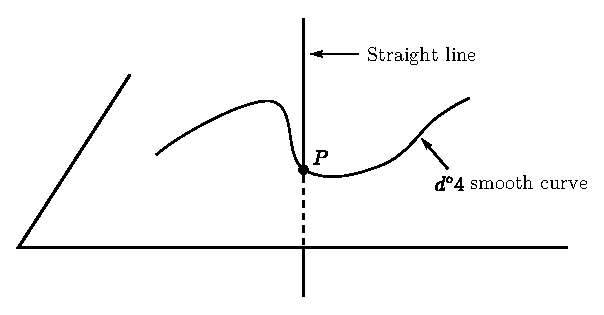
\includegraphics{figure/addfig2.eps}
\end{figure}


If one has Flatness of $X\longrightarrow\Spec V$ as above then
$d^\circ(\mathcal{Z})$ is constant on the family $X$ and for generic
$s$, arithmetic genus of $X(s)=$ arithmetic genus of $X(s_\circ)=p$
and $\chi(O_{\mathcal{Z}}(n))=nd^\circ(\mathcal{Z})-p+1$ by
$R-R$. Moreover here we have
$d^\circ(\mathcal{Z})=5$. There\pageoriginale exists an exact sequence
$$
0\longrightarrow O_Z\longrightarrow O_C\oplus O_L\longrightarrow O_P
\longrightarrow 0.
$$

So
\begin{gather*}
0\longrightarrow H^0(OZ)\longrightarrow H^0(O_C\oplus O_L)
\longrightarrow H^0(O_P)\longrightarrow H^1(O_Z)---\\
\longrightarrow H^1(O_C\oplus(O_L)\longrightarrow 0.
\end{gather*}

So $\dim H^1(O_Z)=\dim H^1(O_C\oplus O_L)=p$ because
$H^1(O_L)=0$. Since $C$ is a plane curve of $\deg 4$,
$$
p_C=H^1(O_C)=\frac{(4-1)\;(4-2)}{2}=3,
$$
hence $p=3$. 
$$
\chi(O_Z(n))=5n-3+1=5n-2.
$$

Now we claim that if $\mathcal{Z}'$ is a smooth deformation, then
$\mathcal{Z}'$ is a plane curve. Since $d\mathcal{Z}'=5$ and $p=3$
$$
p=\frac{(5-1)\;(5-2)}{2}=6\neq 3.
$$

So this will give us the required contradiction. Let $J$ be the ideal
of $\mathcal{Z}$ We want to,
\begin{align*}
& 0\longrightarrow J(1)\longrightarrow
O_{\mathbb{P}}(1)\longrightarrow O_{\mathcal{Z}}(1)\longrightarrow
0.\\ 
& 0\longrightarrow H^0(J(1))\longrightarrow H^0(O_{\mathbb{P}^3}(1))
\longrightarrow H^0(O_{\mathcal{Z}'}(1)) \dim
H^0(O_{\mathbb{P}^3}(1))=4.\\
&\dim(H^0(O_{\mathcal{Z}'}(1)))-\dim H^1(O_{\mathcal{Z}'}(1))=\deg
O_{\mathcal{Z}'}(1)-p+1\\
&\dim(H^0(O_{\mathcal{Z}'}(1))-\dim H^1(O_{\mathcal{Z}'}(1))=5-3+1=3.
\end{align*}

So\pageoriginale if we show that $H^1(O_{\mathcal{Z}'}(1))=0$ we are
through. But $H^1(\mathcal{Z}',\break O_{\mathcal{Z}'}(1))=H^0(\mathcal{Z}',
\omega_{\mathcal{Z}'}(-1)),d^\circ\omega,=2p-2=4,
d^\circ(\omega_{\mathcal{Z}'}(-1)=d^\circ(\omega_{\mathcal{Z}'})-d^\circ
(\delta_{\mathcal{Z}'}(1))=4-5=-1. H^0(C,\mathcal{L})=0$ if
$\mathcal{L}$ is a line bundle on a smooth connected curve and
$d^\circ\mathcal{L} <0$. 
\end{example*}

\setcounter{section}{1}
\setcounter{propn}{1}
\begin{propn}\label{chap1:prop1.2}
Let $C\hookrightarrow\mathbb{P}^3$ be an equidimensional curve which
is locally a complete intersecion. Then there exist $F_1,F_2,F_3,F_4$
forms in $R=k[X_0,X_1,X_2,X_3]$ such that $\Proj(R/\underline{F})=C$
where $\underline{F}=(F_1,F_2,\break F_3,F_4).R$.
\end{propn}

\begin{proof}
We prove the result by choosing $F_i$'s successively as follows.
\begin{itemize}
\item [1.] Choose $F_1$ such that $C$ is a divisor on the surface
defined by zeros of $F_1$. 

\item [2.] $F_2$ is chosen such that $(F_1,F_2)$ generate the ideal of
  $C$ generically. So ideal generated by $(F_1, F_2)$ is equal to the
  ideal of $C$ at almost all points of $C$.

\item [3.] We choose $F_3$, such that $(F_1,F_3)$ generate the ideal
  of $C$ at those finite number of points of $C$ where $(F_1,F_2)$ is
  not equal to the ideal of $C$ and $V(F_1,F_2,F_3)$ has no one
  dimensional components other than that of $C$.

\item [4.] $F_4$ is chosen such that it does not pass through the zero
  dimensional components of $V(F_1,F_2,F_3)$.
\end{itemize}

We use the following eassy lemmas:

\begin{enumerate}
\item {\bf Serre}. Let $M$ be a vector bundle of rank $r$ on a variety
  $X$. Let $V\subset H^0(X,M)$ be a finite dimensional vector space
  and assume 
\begin{enumerate}
\item $r>\dim X$
\item For all closed points $x\in X$, the map from $V$ to $M\otimes
  k(x)$ is surjective.
\end{enumerate}
\end{enumerate}

Then there is an open non empty zariski set of elements $s\in V$ whose
image in every space $M\otimes k(x)$ is non-zero.

\noindent See: Lectures on Curves on an Algebraic surface by
D. Mumford\break pp.~148. 
\end{proof}

\medskip
\noindent{\textbf{II. Lemma of Devissage (i).}}
 Let\pageoriginale $I,J_i,i=1,\ldots n$ be ideals of a ring $A$ 
and at most two of the $J_i$'s are not prime. If $I\subset
\underset{i=1}{\cup}J_i$ then $I\subset J_i$ for some i.

\medskip
\noindent{\textbf{II. Lemma of Devissage (ii).}}
If $E$ is a vector space over a field $k$ and $\{E_i\}_{i\in I}$
sub-vector spaces of $E$ with $\# I<\# k$, then $E=UE_i\Rightarrow
E=E_i$ for some i.

\begin{enumerate}
\item {\bf Existence of $F_1$.} Let $I$ be the ideal sheaf of the
  curve. Then $I/I^2$ is a vector bundle of rank 2 over $O_C$ by
  assumption. The exact sequence 
\begin{gather*}
I(n)\xrightarrow{\varphi}I/ I^2(n)\longrightarrow 0\quad \text{gives a
map},\\
H^0(\mathbb{P}^3,I(n))\xrightarrow{\varphi}H^0(\mathbb{P}^3),I/I^2(n))
=H^0(C,I/I^2(n)), 
\end{gather*}
for every $n$. Since for large enough $n,I/I^2(n)$ is generated by
sections and $\varphi$ is surjective we conclude that $\Im\varphi$
generates $I/I^2(n)$ for large enough $n$. Since rank $I/I^2>\dim C$,
by $(I)$ we have $F_1\in H^0(\mathbb{P}^3,I(n))$ such that $\varphi
(F_1)$ is nowhere vanishing on $C$. So $C$ lies on the surface $Y$
defined by $F_1=0,\varphi(F_1)$ is nowhere vanishing on $C$ implies
that it can be considered as one of the two generators of $I$ at every
point of $C$. So $I/(F_1)$ which is a sheaf on $Y$ is locally
one-generated and it is clear that the generator is not a zero divisor
at those point. So $C$ is a divisor on $F_1$.
\item Choose $F_2$ as the local equation of $C$ on $Y$ at some
point. So in a neighbourhood of that point $(F_1,F_2)$ generate $I.\ie
(F_1,F_2)$ is generically equal to $I$.

\item Let $P_1,P_2\ldots P_m$ be all the points of $C$ where
$(F_1,F_2)\varsubsetneq I_{P_i}$. Let $V\subset H^0(Y,\frac{I(n)}
{(F_1)})$ for large enough $n$ such that $V$ generates $\frac{I(n)}
{(F_1)}$. Let us denote $\frac{I_{P_i}}{F_1}$ by
$\overline{I}_{P_i}$. Then we have a natural map
$V\xrightarrow{\alpha}\bigoplus\limits_{i=1}^m
\overline{I}_{P_i/m_i{I_{P_i}}}$ where $m_i$ corresponds to the
maximal ideal of $O_{P_i}$. Since $V$ generates $\frac{I}{(F_1)} (n)$
at every point, the composite maps,
$$
V\xrightarrow{\alpha}\bigoplus\limits_{i=1}^m\overline{I}_{P_i}/m_i
\overline{I}_{P_i}\xrightarrow{\beta_i}\overline{I}_{P_i/m_i
{\overline{I}_{P_i}}}
$$\pageoriginale
are all surjective. So $\ker (\beta_i\circ\alpha)\varsubsetneq V$ for
every i. By III,
$\bigcup\limits_{i=1}\ker(\beta_i\circ\alpha)\subsetneqq V$. So in the
natural Zariski topology on $V$, there exists a non-empty open set
$V-\bigcup\limits_{i=1}^m \ker(\beta_i\circ\alpha)=W$ such that for
any $s\in W,\beta_i\circ\alpha(s)\neq 0,\quad\forall_i$.

\indent Let us denote by $R_1,R_2,\ldots R_t$ the one dimensional
components of $V(F_1,F_2)$, other than that of $C$. 

\indent Again we have the map 
$$
V\xrightarrow{\alpha'}\bigoplus\limits_{i=1}^tO_{R_i/{m_{R_i}}}\quad
\text{induced from}\quad O\longrightarrow O_{R_i}
$$
Since image of $V$ in $O_{R_i/{m_{R_i}}}$ generates
$O_{R_i/{m_{R_i}}}$ as $O_{R_i/{m_{R_i}}}$-vector spaces, we find that
as before there exists a non-empty open set $A$ in $V$ such that for
any $u\in A,\alpha'(u)$ has all components non-zero.

\indent Since $A$ and $W$ are non-empty open subsets of $V$, which is
irreducible, $A\cap W\neq\phi$. Let $s\in A\cap W$. $s\in H^0(Y,
\frac{I(n)}{F_1})$. So $s$ comes from a homogeneous polynomial $F_3\in
I$. Since $\beta_i\circ\alpha(s)\neq 0$ and $\overline{I}_{P_i}$ is
one generated we see that $\beta_i\circ\alpha(s)$ is generated by
$\beta_i\circ \alpha(s)\ie (F_1,F_3)_{P_i}=I_{P_i}\;\forall
P_i$. Again we see that since $\alpha'(s)\neq 0$ in every one of the
$O_{R_i/{m_{R_i}}}, (F_1,F_3)_{R_i}=O_{R_i}\ie R_i$'s are not
components of this variety. So we have, 
$$
(F_1,F_2,F_3)_P=I_P\quad\text{at every}\quad P\in C.
$$

The only irreducible components of $V(F_1,F_2,F_3)$ are components of
$C$ and finitely many closed points.
\item We choose $F_4\in I$ which does not vanish at these zero
  dimensional components. 
So one has $F_1,F_2,F_3,F_4$ which generate $I$ on $\mathbb{P}^3$.
\end{enumerate}

\begin{REM*}
There\pageoriginale exist smooth curves (in particular, locally
complete intersection) in $\mathbb{P}^3$ which are not ideally defined
by three equations. See: Corollary~ 7.2, Liaison des varietes
algebriques. I, by C. Peskine and L. Szpiro. Inventiones Math. (26, 1974. 
\end{REM*}

